\documentclass[twocolumn,superscriptaddress, prl,showpacs]{revtex4-1}
\setlength{\parskip}{0mm }
\setlength{\belowcaptionskip}{-10pt}
\usepackage{amsfonts}
\usepackage{amssymb}
\usepackage{amsmath}
\usepackage{amsthm}
\usepackage{dsfont}
\usepackage[dvipdfm]{graphicx}
\usepackage{stackrel}
\usepackage{color}

% Should come last b/c it needs to overload a bunch of commands
\usepackage{hyperref}

\newcommand{\ket}[1]{|#1\rangle}
\newcommand{\bra}[1]{\langle #1 |}
\newcommand{\be}{\begin{equation}}
\newcommand{\ee}{\end{equation}}
\newcommand{\addr}[1]{\textcolor{red}{#1}}


\begin{document}
\title{Slowest local operators in quantum spin chains}

\author{Hyungwon Kim}
\affiliation{Physics Department, Princeton University, Princeton, NJ 08544, USA}
\affiliation{Department of Physics and Astronomy, Rutgers University, Piscataway, NJ 08854, USA}

\author{Mari Carmen Ba\~{n}uls}
\affiliation{Max-Planck-Institut f$ {\ddot{u}}$r Quantenoptik, Hans-Kopfermann-Str. 1, 85748 Garching, Germany}

\author{J. Ignacio Cirac}
\affiliation{Max-Planck-Institut f$ {\ddot{u}}$r Quantenoptik, Hans-Kopfermann-Str. 1, 85748 Garching, Germany}

\author{Matthew B. Hastings}
\affiliation{Station Q, Microsoft Research, Santa Barbara, CA 93106-6105, USA}
\affiliation{Quantum Architectures and Computation Group, Microsoft Research, Redmond, WA 98052, USA}

\author{David A. Huse}
\affiliation{Physics Department, Princeton University, Princeton, NJ 08544, USA}

\begin{abstract}
We numerically construct slowly relaxing local operators in a nonintegrable spin-1/2 chain.
Restricting the support of the operator to $M$ consecutive spins along the chain,
we exhaustively search for the operator that minimizes the Frobenius norm of the commutator
with the Hamiltonian and show that the Frobenius norm bounds the time scale of relaxation of the operator 
at high temperatures.
We find operators with significantly slower relaxation than
the slowest simple ``hydrodynamic'' mode due to energy diffusion.
Using both exhaustive search and tensor network techniques, we find
similar slowly relaxing operators for a Floquet spin chain; % and for quantum circuits on spin chains;
this systems is hydrodynamically ``trivial'', with no conservation laws restricting their dynamics.
We argue that such slow relaxation may be a generic feature following from locality and unitarity.
\end{abstract}

\pacs{05.30.-d, 05.70.Ln}

\maketitle

It has been proposed that an isolated quantum many-body system can still thermalize, in the sense that local observables approach their thermal equilibrium values \cite{Deutsch:1991,Srednicki:1994,Rigol:2008}.  The presence of additional conserved quantities leads to relaxation to a generalized ensemble \cite{Rigol:2007,Calabrese:2011,Gogolin:2011,Fagotti:2014}.  Experimental studies have increased the interest in these questions \cite{Polkovnikov:2011, Yukalov:2011}.  One proposed theoretical explanation is the eigenstate thermalization hypothesis (ETH) \cite{Deutsch:1991,Srednicki:1994,Rigol:2008,Santos:2010,Rigol:2012,Kruczenski:2013,Beugeling:2014,Sorg:2014,Kim_ETH,Goldstein:2014}, which argues that many-body eigenstates of thermalizing nonintegrable Hamiltonians have local reduced density operators that are thermal; then, at long times, dephasing between different energy eigenstates brings small subsystems to thermal equilibrium.

However, not all systems show this local thermalization in an accessible time scale \cite{Banuls:2011}.
One possibility is that the ETH is false for the system of Ref.~\onlinecite{Banuls:2011}; another possibility is that the time scales required to thermalize locally are too long to be numerically accessible.  A question is: how can such slow thermalization arise, when a nonintegrable system like the one studied has no conserved local quantities other than energy?

In this work, we illustrate how such slow relaxation can emerge by showing that indeed slow, almost-conserved local quantities {\it are} present in many nonintegrable systems.  We construct these operators numerically, by explicitly searching for operators with a small commutator with the Hamiltonian.
One of such operators with a small commutator is the one that results from the thermal diffusion due to a spatially-smooth inhomogeneity in the energy density.  However, we show numerically that these are {\it not} the operators with the smallest commutator.  Instead, other operators are present with a much smaller commutator.  Thus we find ``unexpected almost-conserved quantities" for these systems.  For numerical reasons discussed below, much of our work focuses on the Frobenius norm rather than operator norm to measure relaxation, but we also discuss the operator norm.


We also construct the pattern of local energy density that gives the slowest operator of that form.  This operator and its commutator with the Hamiltonian
match the expectations from diffusive hydrodynamics, with the square of the Frobenius norm of the commutator $\sim M^{-2}$ for the slowest such operator on a subregion containing $M$ spins.
However, numerically we observe that the commutator for the slowest operator that we find by exhaustive unrestricted search appears to decrease with a {\it larger} power of length than this diffusive $\sim M^{-2}$, and for the accessible system sizes is quantitatively substantially smaller (slower) than that of the simple diffusive mode.

To further understand the presence of such approximately conserved quantities we then turn to a Floquet spin chain where energy is not conserved.
We also find slowly relaxing operators in this Floquet system.
%To test this, we also consider several random unitaries constructed from local quantum circuits, and in every case we again find slowly relaxing operators.
In fact, we argue that some slowly relaxing operators must be present in any Floquet system or \addr{more generally} in any quantum circuit.
However, these slowly relaxing operators are in a sense morally similar to the slowly relaxing operator in a Hamiltonian system describing energy fluctuations: these slow operators are present in any such system, so long as the unitary dynamics is local.  They themselves do not inhibit relaxation of the local density matrices ``as fast as possible" i.e., on a time scale proportional to the length of the interval;
(see Ref.~\onlinecite{Brandao:2012} for a proof that this happens for random local circuits).
Thus, the real surprise is our numerical observation that there are other operators in some nonintegrable Hamiltonian systems (and possibly in some quantum circuits) with even slower relaxation.



\begin{figure}
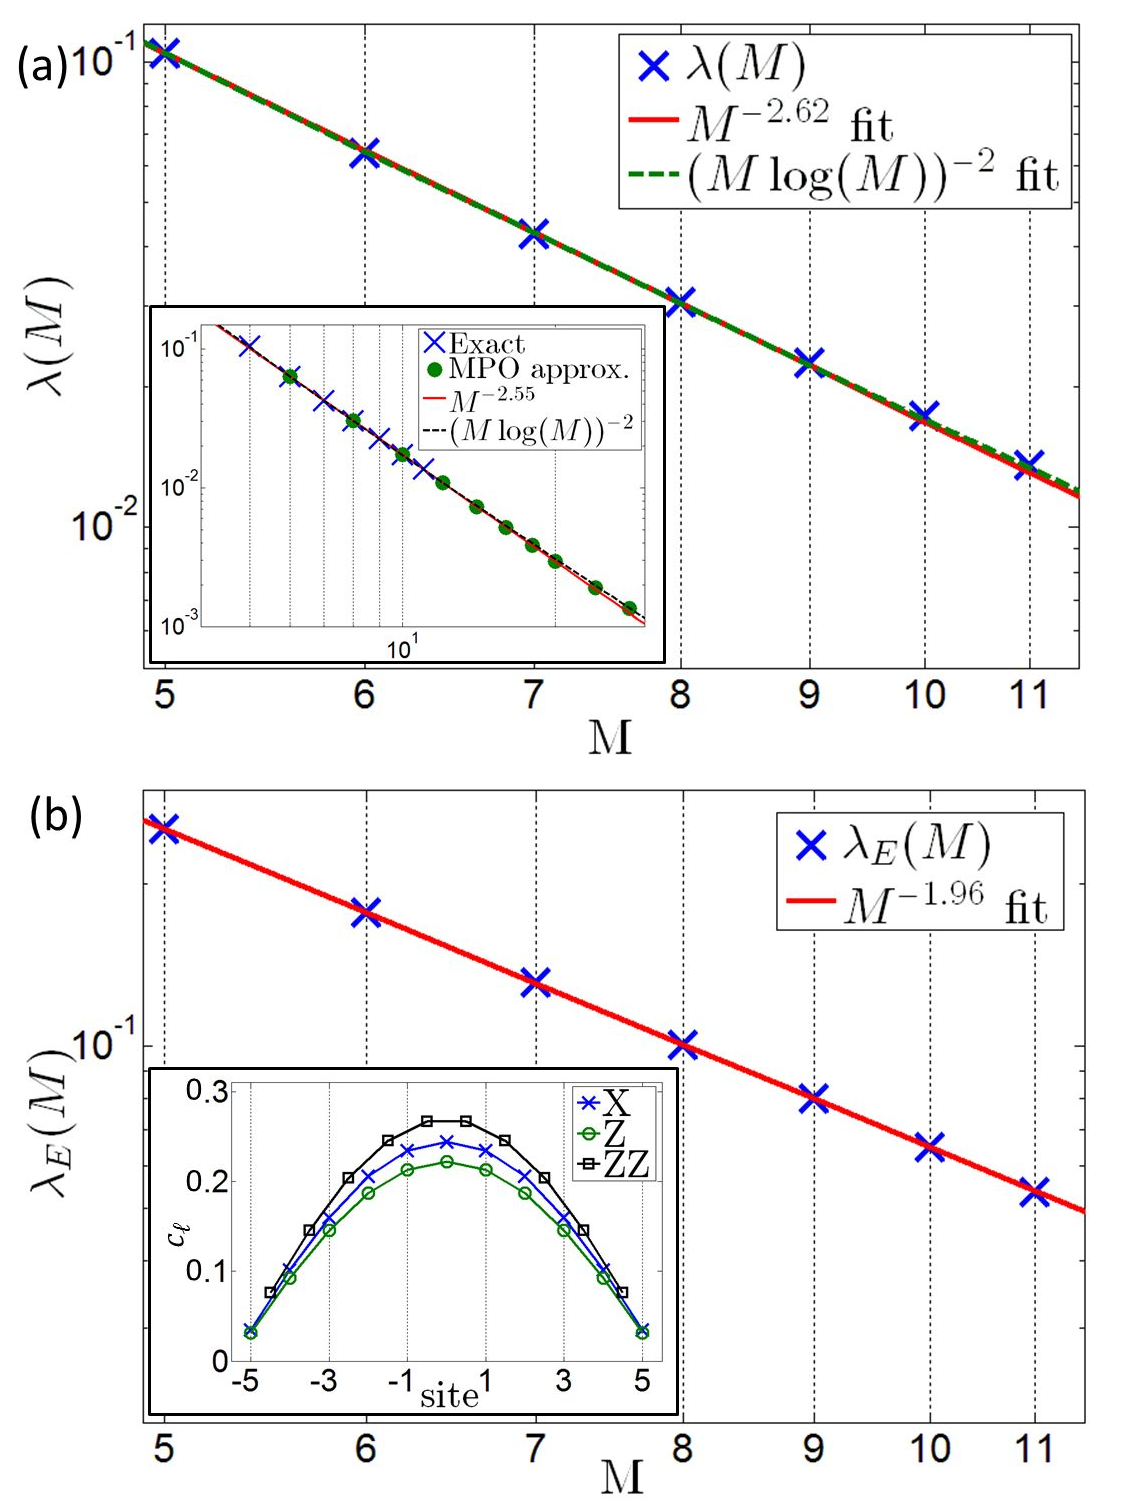
\includegraphics[width=0.95\linewidth]{fig_hamiltonian_modified.pdf}
\centering
\caption{(color online) (a) $\lambda(M)$ is the minimum of Eq. \eqref{eq:minimize}.  As we increase $M$, the commutator with the Hamiltonian decreases as shown.
This decrease can be well-fitted by either a power-law or $1/(M\log(M))^2$. \addr{Inset: $\lambda(M)$ vs. $M$ using tensor network method (MPO approximation). The results are indistinguishable with available exact results. The exponent of power-law fitting slightly changes but the main result holds.} 
(b) $\lambda_E(M)$ is the minimum of Eq. \eqref{eq:minimize} when only terms in the Hamiltonian are used.  As thermal diffusion suggests, it decreases as $1/M^2$. Inset: Structure of the optimal operator for $M = 11$. $X$, $Z$, and $ZZ$, are
abbreviations of $\sigma^x_\ell$, $\sigma^z_\ell$, and $\sigma^z_\ell \sigma^z_{\ell+1}$, respectively.
We locate the $\sigma^z_\ell \sigma^z_{i+1}$ term at $\ell+1/2$.  The coefficients are normalized to have unit square norm ($\sum_\ell c_\ell^2 = 1$).
It shows a clear sinusoidal energy modulation with the expected wavelength $2M$, and with the relative ratios equal to those in the Hamiltonian.}
\label{fig:hamiltonian}
\end{figure}


{\it Hamiltonian System Numerical Results---}
As a nonintegrable model Hamiltonian, we choose a spin-1/2 Ising chain with both longitudinal and transverse fields:
\begin{align}
H = \sum_{i = -\infty}^{\infty} g\sigma^x_i + h\sigma^z_i + \sigma^z_i \sigma^z_{i+1} ~,
\label{eq:Hamiltonian}
\end{align}
where $\sigma^x_i$ and $\sigma^z_i$ are Pauli matrices of the spin at site $i$.
Ref.~\onlinecite{Banuls:2011} has found a nonthermalizing state for this model within the accessible time scale.
We choose $(g,h) = (0.905, 0.809)$, at which this model is known to be robustly nonintegrable even for a relatively small system size \cite{Kim:2013}.
See supplemental for another choice of parameters.

We consider local operators supported on a finite interval of $M$ consecutive sites.
For simplicity, we do not assume translation invariance
\footnote{We have also performed similar analysis in the infinite chain with translation invariance so the action of the local operator is the same on all sites. Most of our main results (Figures \ref{fig:hamiltonian} (a), \ref{fig:floquet} (a), and \ref{fig:random_circuit})
remain true. Since it is easier to visualize the local operators and to directly compare with diffusive energy mode in a translationally non-invariant system, we present the results on an infinite chain where the local operator is placed on $M$ specific consecutive sites.}.
Every traceless Hermitian operator
$\hat{A}_M$ can be expressed by a linear combination of $4^M - 1$ traceless Hermitian basis operators (excluding the identity).
Therefore, we write
\begin{align}
\hat{A}_M = \sum_{\ell = 1}^{4^M - 1} c_\ell \hat{O}_{(M,\ell)} ~,
\end{align}
where $c_\ell$ is a real number and $\hat{O}_{(M,\ell)}$ is the corresponding basis operator.
We choose $\hat{O}_{(M,\ell)}$ to be mutually orthogonal using the Hilbert-Schmidt inner product so that
$\mathrm{tr(\hat{O}_{(M,\ell)} \hat{O}_{(M,k)})} = 0$ for $\ell\neq k$.

The dynamics of an operator comes from the commutator with Hamiltonian.
Therefore, we want to {\it minimize} the magnitude of $[\hat{A}_M, H]$
to construct a slowly relaxing local operator of length $M$.
%Using the square of the Frobenius norm, $\mathrm{tr(\hat{O}\hat{O}^\dag)}$, to measure this magnitude\footnote{There are three widely used norms of an operator;
%the operator norm (largest absolute eigenvalue of the operator), the trace norm ($\mathrm{tr(\sqrt{\hat{O}\hat{O}^\dag})}$),
%and the Frobenius norm ($\sqrt{\mathrm{tr(\hat{O}\hat{O}^\dag)}}$). Each norm has its own meaning.
%Although the operator norm is physically the most relevant one for our purpose,
%we choose the Frobenius norm since it is the easiest to numerically optimize.
%See supplementary material for details of the relevance of the operator norm.},
\addr{We use the square of the Frobenius norm, $\mathrm{tr(\hat{O}\hat{O}^\dag)}$, to quantify the commutator 
since it gives a quadratic form  (Eq. \eqref{eq:minimize}) of which we can readily find the minimum. 
Although the operator norm generally controls the dynamics at arbitrary time, its numerical minimization is very challenging 
\footnote{\addr{We can get the upper bound of the operator norm by using the operators that minimize the Frobenius norm. 
The behavior of upper bounds is consistent with the results we obtained using the Frobenius norm. 
See supplementary material for details.}}, and the (square of) Frobenius norm can actually bound the thermalization time scale at infinite temperature,
where we expect dynamics is fastest, as we show below.} 

We minimize the following:
\begin{align}\label{eq:minimize}
f(\hat{A}_M) &= \frac{\mathrm{tr([\hat{A}_M,H][\hat{A}_M,H]^\dag)}}{\mathrm{tr(\hat{A}_M\hat{A}^\dag_M)}} \nonumber\\
&= \sum_{\ell,k}\frac{c_\ell c_k \mathrm{tr([\hat{O}_{(M,\ell)},H][\hat{O}_{(M,k)},H]^\dag)}}{\sum_j c_j ^2 \mathrm{tr((\hat{O}_{(M,j)})^2)}} ~.
\end{align}
We define $\lambda(M)$ to be the minimum of $f(\hat{A}_M)$:
%\begin{align}
$\lambda(M) = \mathrm{min}\{f(\hat{A}_M)\}$,
%\end{align}
and we call the corresponding $\hat{A}_M$ the slowest operator acting on $M$ sites.
Since the Hamiltonian has time-reversal symmetry,
we can consider even and odd operators under time-reversal separately.
It turns out that for $M\geq 4$, the minimizer of $f(\hat{A}_M)$ always comes from the even sector.
\addr{Up to $M = 11$, we obtain exact results and up to $M = 28$, we use tensor network method (approximating operators by matrix product operators (MPO)).
The MPO results have converged within 1$\%$ with bond dimension 140 \footnote{\addr{How such a small bond dimension is sufficient remains unclear.} }.}

First, let's understand the physical meaning of this quantity.
We consider an initial mixed state $\rho = I/Z + \epsilon \hat{A}_M$, % such as
%\begin{align}\label{eq:initial}
%\rho = \frac{1}{Z}I + \epsilon\hat{A}_M ~,
%\end{align}
where $Z$ is the normalization factor, $I$ is the identity and $\epsilon$ is chosen to make $\rho$ nonnegative.
$\hat{A}_M$ serves as a small inhomogeneity in the infinite temperature ensemble and
is assumed to have unit Frobenius norm.
Let's define $a_M(t)$ as the expectation value of $\hat{A}_M/\epsilon$ at time $t$:
$a_M(t) = (1/\epsilon)\mathrm{tr}(\rho \hat{A}_M(t)) = \mathrm{tr}(\hat{A}_M \hat{A}_M(t))$,
where $\hat{A}_M(t)$ is in the Heisenberg picture. [Note that $a_M(0) = 1$.]
Using Cauchy-Schwarz inequality, we can show the following:
\begin{align}
\left|\frac{d^2 a_M(t)}{dt^2}\right| = |\mathrm{tr}([\hat{A}_M(t),H][\hat{A}_M,H])| \leq f(\hat{A}_M) ~,
\label{eq:second_derivative}
\end{align}
Therefore, we can bound the distance between $a_M(t)$ and $a_M(0)$.
\begin{align}
|a_M(t) - a_M(0)| = \left|\int^t_0 d\tau \int^\tau_0 d\tau' \frac{d^2 a_M(\tau')}{d\tau'^2}\right| \leq \frac{f(\hat{A}_M) t^2}{2} ~.
\end{align}
In thermodynamic limit and finite $M$, the thermal expectation value is
$a_M^{th} = \rm{tr}(\hat{A}_M) = 0$.
Now we have the following inequality:
\begin{align}
|a_M(t) - a_M^{th}| &\geq |a_M(0) - a_M^{th}| - |a_M(0) - a_M(t)|  \nonumber\\
& \geq 1 - \frac{f(\hat{A}_M)t^2}{2} ~.
\label{eq:hamiltonian_timescale}
\end{align}
Consequently, $f(\hat{A}_M)$ is a lower bound of the thermalization time scale $\tau$ of $\hat{A}_M$ by $\tau \geq f(\hat{A}_M)^{-1/2}$,
and small $\lambda(M)$ implies a long thermalization time scale of the corresponding $\hat{A}_M$.
In addition, since $\lambda(M)$ is the minimum of Eq. \eqref{eq:second_derivative} at $t =0$,
the optimal $\hat{A}_M$ is {\it the} slowest operator at early time.


Figure \ref{fig:hamiltonian} (a) plots $\lambda (M)$.
It is clear that $\lambda(M)$ decreases with $M$ as it should.
The data can be well-fitted by two functional forms; power-law decay with exponent $2.62$ and a logarithmic correction to $1/M^2$, which is $1/(M\log(M))^2$.
In either case, the rate of decrease with $M$ is {\it faster} than $1/M^2$, which is the scaling of the slowest diffusive energy mode as we show now.

{\it Hydrodynamics---}
A slowly relaxing energy mode can be constructed by considering an energy modulation of wavelength $2M$:
\begin{align}
\hat{E}_M = \sum_i c_M(i) h_i
&= \sum_{i=-M/2}^{M/2} \cos\left(\frac{i\pi}{M}\right)(g \sigma^x_i + h\sigma^z_i)\nonumber\\
&\quad+ \sum_{i=-M/2}^{M/2-1} \cos\left(\frac{(i+1/2)\pi}{M}\right)\sigma^z_i\sigma^z_{i+1} ~,
\label{eq:energy_modulation}
\end{align}
where $h_i$ is the energy density operator ($g \sigma^x_i + h\sigma^z_i + 1/2(\sigma^z_{i-1}\sigma^z_i + \sigma^z_i\sigma^z_{i+1}$))
and $c_M(i)$ is the cosine modulation function restricted to lie in $[-M/2,M/2]$.
Since the energy is conserved, we can use the continuity equation:
$d h_i/dt = -\nabla \cdot {\bf j}_i$, where ${\bf j}_i$ is the energy current density at site $i$:
${\bf j}_i = g(\sigma^y_i \sigma^z_{i+1} - \sigma^y_{i+1} \sigma^z_i)$.
Combining this with the Heisenberg equation of motion, we have the following.
\begin{align}
 i[H,\hat{E}_M] &= \frac{d}{dt} \hat{E}_M = -\sum_i c_M(i) \partial_i \cdot {\bf j}_i \\
 &= \sum_i {\bf j}_i \partial_i c_M(i) \simeq -\frac{\pi}{M} \sum_i s_M(i) h_i,
\end{align}
where $\partial_i$ is the discrete spatial derivative and $s_M(i)$ is the sine modulation.
Therefore, $\mathrm{tr}([H,\hat{E}_M][H,\hat{E}_M]^\dag) \sim 1/M^2$.

Here, we adapt a more conservative approach.
We do the same numerical search as before but restrict the operator space within the terms in the Hamiltonian
so we only consider $3M-1$ basis operators instead of $4^M-1$.
Figure \ref{fig:hamiltonian} (b) plots $\lambda_E(M)$, the minimum of $f(\hat{A}_M)$ in this restricted space.
As expected, we have almost perfect $1/M^2$ scaling.
Since there are only a few basis operators, we can easily look at the details of the structure of the optimal operator.
The inset of Figure \ref{fig:hamiltonian} (b) is the structure of the optimal operator in terms of the local terms in Hamiltonian.
It is indeed the form of Eq.~\eqref{eq:energy_modulation} and thus the energy modulation of the longest wavelength is the slowest energy mode.
Note also the fact that apart from displaying a different scaling, $\lambda(M)$ is much smaller than $\lambda_E(M)$. 
%\addr{We have also used a tensor network method, restricting the bond dimension to 4 (only on-site and nearest-neighbor terms are allowed), 
%and obtained exactly the same results.}  

{\it Floquet System---}
Next, we consider a Floquet system (for thermalization in the Floquet system, see Refs.~\onlinecite{Dalessio:2014, Lazarides:2014, Ponte:2014}) and test whether the energy conservation is important in the slow relaxation of local operators.
We adopt the same Floquet operator used in Ref.~\onlinecite{Kim_ETH}:
\begin{align}
U_F = \exp(-i H_x \tau) \exp(-i H_z \tau) ~,
\label{eq:floquet_op}
\end{align}
where $H_x$ is the $\sigma^x$ part ($\sum_i g \sigma^x_i$) and $H_z$ is the $\sigma^z$ part ($\sum_i h \sigma^z_i +\sigma^z_i \sigma^z_{i+1}$)
of the Hamiltonian. We choose $\tau = 0.8$.
Although $U_F$ does not conserve energy, it acts {\it locally} on the system.
This type of Floquet operator is shown to thermalize a local operator to the infinite temperature ensemble \cite{Kim_ETH,Prosen:2002}.

We minimize the square of the Frobenius norm of the commutator with the Floquet operator.
%This time we use a Lanczos method to find the $2^M \times 2^M$ matrix $\hat{A}_M$ up to $M = 11$ and a tensor network method for $M = 12, 14, 16$
\addr{Up to $M = 11$, we obtain exact results and up to $M = 16$, we use a tensor network method to find the minimum of the following
\footnote{\addr{The results have converged with bond dimension 260.}}:}
%that minimizes \footnote{Unlike the Hamiltonian, the Floquet operator makes the matrix of dimension $4^M-1$ in Eq. \eqref{eq:minimize} dense and thus
%limits the largest $M$ that can be explored by the same method to 8. A Lanczos method enables us to access at least up to $M = 11$ exactly.
%Using a tensor network method, we obtain convergent results with bond dimension of order 200 up to $M$ = 16.}:
\begin{align}\label{eq:floquet_minimize}
g(\hat{A}_M) = \frac{\mathrm{tr}([\hat{A}_M,U_F][\hat{A}_M,U_F]^\dag)}{\mathrm{tr}(\hat{A}_M\hat{A}_M^\dag)} ~.
\end{align}
Again, we define $\lambda(M) = \mathrm{min}\{g(\hat{A}_M)\}$ and
call the corresponding $\hat{A}_M$ the slowest operator.

Let's relate $g(\hat{A}_M) $ with the thermalization time scale.
As in the case of Hamiltonian system, we consider the same initial state; $\rho = I/Z + \epsilon \hat{A}_M$. %Eq. \eqref{eq:initial}.
Since the time step in the Floquet system is discrete, we define $a_M^{(N)} = \mathrm{tr}(\hat{A}_M(N)\hat{A}_M )$, with
$a_M^{(0)} = 1$ and $\hat{A}_M(N) = U_F^{\dag N}\hat{A}_M U_F^N$. Using Cauchy-Schwarz inequality, we can show that
\begin{align}
|a_M^{(n+1)} - a_M^{(n)}| = |\mathrm{tr}([\hat{A}_M(N),U_F]\hat{A}_M U_F^{\dag})| \leq \sqrt{g(\hat{A}_M) } ~.
\end{align}
Then, the following inequality follows:
\begin{align}
|a_M^{(N)} - a_M^{0}| %&= \left|\sum_{n=0}^{N-1}a_M^{(n+1)} - a_M^{(n)}\right| \nonumber\\
\leq \sum_{n = 0}^{N-1}|a_M^{(n+1)} - a_M^{(n)}| \leq N \sqrt{g(\hat{A}_M) } ~.
\end{align}
In case of the Floquet system, the thermal expectation value $\hat{a}_M$ is indeed zero and thus
\begin{align}
|a_M^{(N)} - a_M^{th}| \geq |a_M^{(0)}| - |a_M^{(N)} - a_M^{(0)}| \geq 1 - N \sqrt{g(\hat{A}_M) } ~.
\label{eq:floquet_timescale}
\end{align}
This proves that $g(\hat{A}_M)$ is a lower bound of the thermalization time of $\hat{A}_M$ by
$N \geq g(\hat{A}_M) ^{-1/2}$. Again, small $\lambda(M)$ implies a long thermalization time.


\begin{figure}
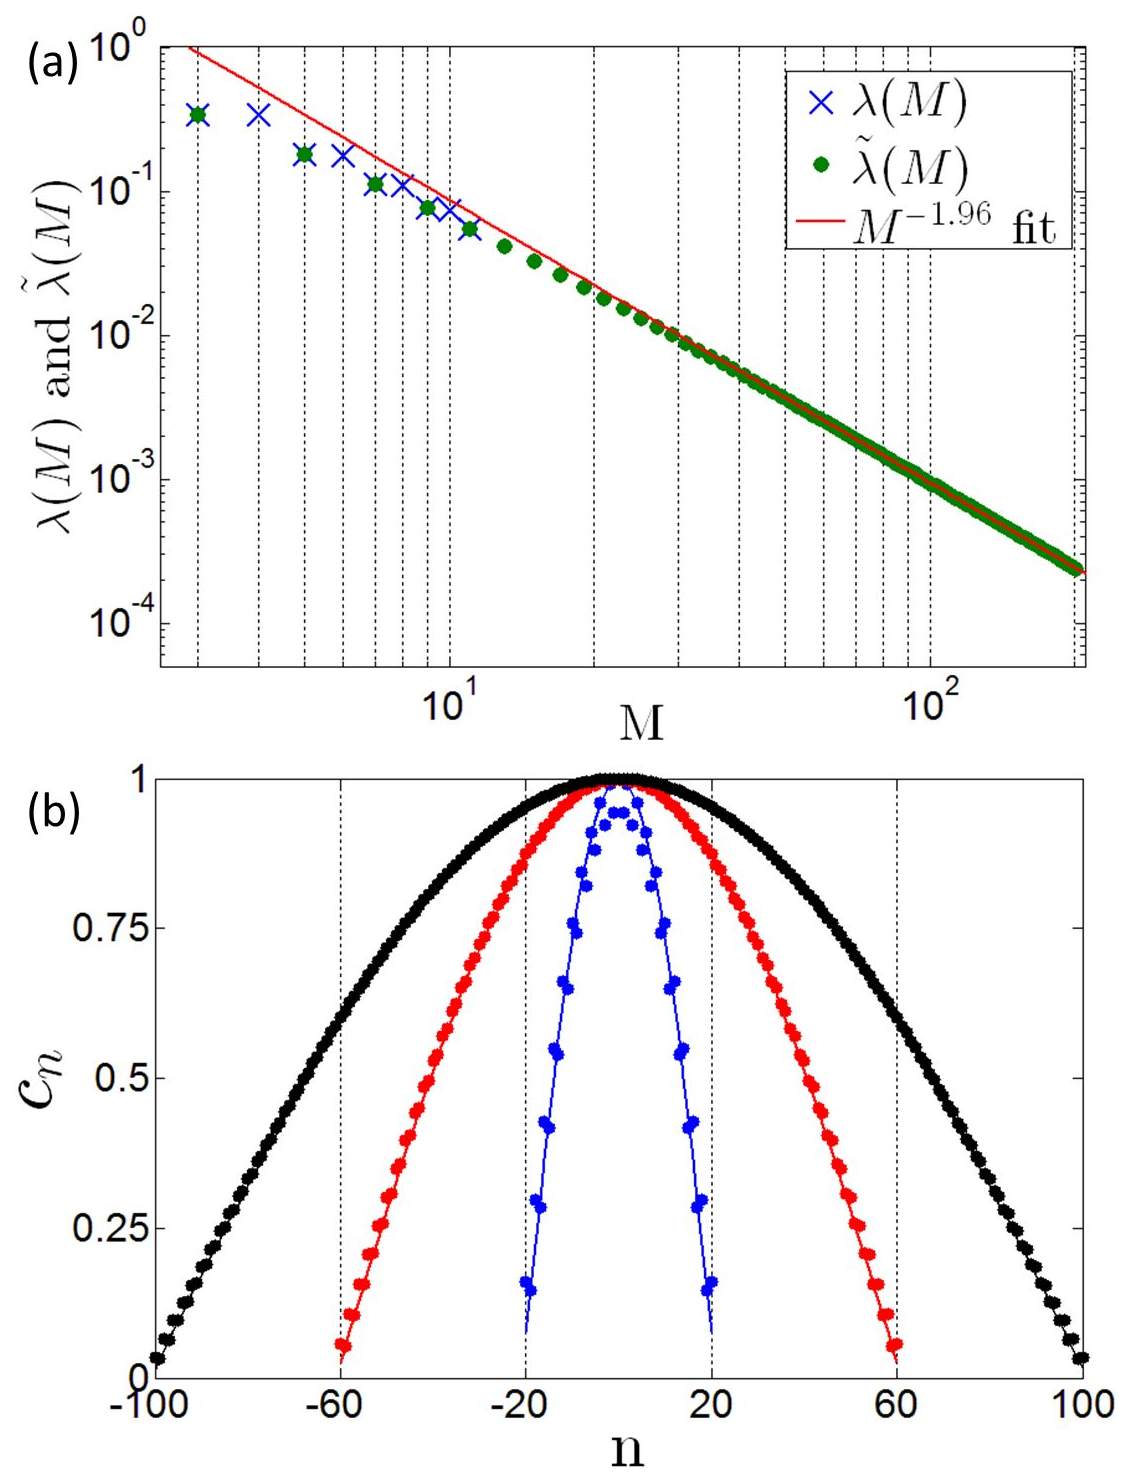
\includegraphics[width=0.95\linewidth]{fig_floquet.pdf}
\centering
\caption{(color online) (a) $\lambda(M)$ (blue X) is the exact minimum from exhaustive search and $\tilde{\lambda}(M)$ (green dot) is a variational upper bound found in the form of Eq. \eqref{eq:filter}. The fractional difference between $\lambda(M)$ and $\tilde{\lambda}(M)$ is less than 1/200 for $M$ = 3,5,7,9, and 11. $\tilde{\lambda}(M)$ decreases close to $M^{-2}$ asymptotically. Note that there is a strong parity effect in the exact result: $\lambda(2N-1) \simeq \lambda(2N)$.
(b) Structure of coefficients $c_n$ (dots) for $N$ = 20 (blue, most narrow), 60 (red, intermediate width), and 100 (black, widest). They all can be well fitted by a cosine function with wavelength $4N+2$ (solid lines) except near $n = 0$ of $N = 20$. }
\label{fig:floquet}
\end{figure}


To extend to larger systems, we use a tensor network technique and assume a specific form of the optimal operator.
We consider operators in the space spanned by $U^n \hat{O} U^{- n}$ for $\hat{O}$ a traceless hermitian operator acting on a single site
and taking a finite number of powers of unitary operator $U$ (this case, the Floquet $U_F$).
Considering the operator of the following {\it filtered} form,
\begin{align}
 \tilde{A}_N=\sum_{n=-N}^N c_n U^n \hat{O} U^{- n} ~,
 \label{eq:filter}
\end{align}
where $\tilde{A}_N$ is supported on $M = 2N+1$ sites for the Floquet system,
we find $\tilde{A}_N$ that gives $\tilde{\lambda}(M) = \mathrm{min}\{\mathrm{tr}([\tilde{A}_N,U][\tilde{A}_N,U]^\dag)/\mathrm{tr}(\tilde{A}_N\tilde{A}_N^\dag)\}$
by varying the coefficients $\{c_n\}$ and $\hat{O}$.
This method can be considered as a version of the Lanczos method as it also works in a Krylov subspace,
but here we use a tensor network method to approximate the traces ${\rm tr}(\hat{O}^\dagger U^n \hat{O} U^{-n})$. %needed to compute the ratio in Eq.~(\ref{eq:floquet_minimize}). 
All data %(including the random circuit case we discuss below) 
have well converged at the bond dimension 80.
Thus $\tilde{\lambda}$ is a variational upper bound of the true minimum $\lambda$.
Interestingly, this simple model \addr{with only 2$N$ + 4 real variables ($2N+1$ for $c_n$'s and 3 for $\hat{O}$)}
%\footnote{there are only 2$N$+ 4 real variables ($2N+1$ for $c_n$'s and 3 for $\hat{O}$) instead of $4^{2N+1} - 1$ variables
%in the case of the exhaustive search.}
agrees very well with the \addr{available exact results ($M =11$ or $N = 5$).}
%exact search until $M = 11$ ($N = 5$), the largest size accessible by an exact method. %which is the largest accessible size by the Lanczos method.
Moreover, we find that the filtered $\hat{A}_N$ that gives $\tilde{\lambda}(M)$
is obtained from the same single site operator $\hat{O}$ for all values of $N$.
For the given model and the parameters, $\hat{O} = 0.04\sigma^x  - 0.66\sigma^y + 0.75\sigma^z$.
Note that $\tilde{A}_N$ can only be supported on odd number of sites.
It turns out that the exact operator of even support can be approximated by a simple symmetric extension:
$\tilde{A}_N\otimes \sigma^0 + \sigma^0\otimes\tilde{A}_N$, where $\sigma^0$ is an identity.
Therefore, $\lambda(2N-1) \simeq \lambda(2N)$.


Figure \ref{fig:floquet} (a) is the plot of $\lambda (M)$, the minimum value of Eq. \ref{eq:floquet_minimize}, and
$\tilde{\lambda}(M)$, which was obtained by the form of Eq. \eqref{eq:filter}.
$\tilde{\lambda}(M)$ asymptotically decreases very close to $M^{-2}$
and its optimal distribution of $\{ c_n\}$ is close to a cosine modulation (Figure \ref{fig:floquet} (b)),
which \addr{we expect to be a generic feature of quantum circuits with local dynamics 
\footnote{\addr{See supplementary material.}}.} %re-appears in a random circuit model we study later.

Comparing Figure \ref{fig:floquet} (a) with Figure \ref{fig:hamiltonian} (a),
we see that $\lambda(M)$ decreases {\it slower} than Hamiltonian cases, which indicates that the Floquet system thermalizes
the local operator {\it faster}. Since the only apparent difference between the Hamiltonian system and the Floquet system
is the existence of the energy conservation, we attribute this faster relaxation to the absence of conservation law.
Nevertheless, Figure \ref{fig:floquet} clearly exhibits that the rate of relaxation in the Floquet system
becomes slower as the support $M$ increases, thus $\hat{A}_M$ is again an approximately conserved quantity.

Such a decay $1/M^2$ would be exact with a cosine if
${\rm tr}(\hat{O} U^n \hat{O} U^{- n})=0$ for all $n \neq 0$.
We are unable to prove this decay in general but show weaker results in the supplemental.
Finally, we do not preclude the possibilities that
there might be \addr{some quantum systems without local conservation law where} 
operators $\hat{A}_M$ with $\lambda(M)$ decreas even faster than $1/M^2$,
which would be very interesting.


{\it Summary---}
We have numerically constructed a series of local operators that relax slower than local energy fluctuations do.
We have also performed the same analysis in the similar system without energy conservation,
the Floquet system and for a family of quantum circuits, again finding slowly relaxing operators.
The structure of the operators found turns out to be very complicated, involving all basis operators
(if we restrict to just the terms in the Hamiltonian, we only obtain simpler operators related to energy currents),
and so their origin remains unclear.
These operators present a new class of observables; if they can be studied experimentally, they may reveal unsuspected slow relaxation.

{\it Acknowledgement---}We thank Fabian Essler for stimulating discussions and Stefan K\"{u}hn for help in numerical algorithms.
H.K. is grateful for the support and hospitality of Max-Planck-Institute f\"{u}r Quantenoptik,
where this work has begun and Korea Institute for Advanced Study, where part of this manuscript was written.
MCB and JIC were partially funded by the EU through the SIQS integrated project.


\bibliography{slow_op_bibl}

\newpage
\section*{Supplementary Material}

\subsection{Operator Norm}
In the main text, we have used the square of the Frobenius norm to quantify the commutator with the Hamiltonian
and related it to the time scale of thermalization of the local operator.
In this section, we use the operator norm (the largest eigenvalue in magnitude),
to estimate the thermalization time scale.


Let us assume that $\hat{A}_M$ satisfies the following:
\begin{align}
||[\hat{A}_M, H]|| \leq \chi(M),
\end{align}
where $H$ is the Hamiltonian and $||\ldots||$ means the operator norm of the argument and $\chi(M)$ is some nonnegative valued function.
Then, using the Heisenberg equation of motion, we have
\begin{align}
\bigg|\bigg|\frac{d}{dt} \hat{A}_M(t)\bigg|\bigg| &= \bigg|\bigg| e^{-i H t} \left(\frac{d}{dt} \hat{A}_M (t)\right) e^{i H t} \bigg|\bigg| \nonumber\\
&= ||[\hat{A}_M(t = 0), H]|| \leq \chi(M) \\
||\hat{A}_M(t) - \hat{A}_M(0)|| &= \bigg|\bigg|\int_0^t \left(\frac{d}{d\tau} \hat{A}_M(\tau)\right)d\tau \bigg|\bigg| \nonumber\\
&\leq \int^t_0 \big|\big|\frac{d}{d\tau} \hat{A}_M(\tau)\big|\big|d\tau \leq \chi(M) t ~,
\end{align}
where we have used the fact that $e^{-iHt}$ is a norm-preserving unitary operator.
This inequality bounds the distance of an operator evolving under Hamiltonian dynamics
from its initial configuration. 
\addr{Note that we used the {\it square} of the Frobenius norm to bound the distance 
from the thermal value in the main body, where we find the bound of the thermalization time is given by $\sqrt{\lambda(M)}$.}


Next, we consider an initial state $\rho$ such that
\begin{align}
|\langle \hat{A}_M \rangle_0 - \langle \hat{A}_M \rangle_\beta| = \gamma(M) ~,
\end{align}
where $\langle \ldots \rangle_0$ is the expectation value of the initial condition, $\langle \ldots \rangle_\beta$
is thermal expectation value and $\gamma(M)$ is some nonnegative valued function.
Now we can estimate the distance between the thermal expectation value and the expectation value at time $t$ (for $t \leq \gamma(M)/\chi(M)$):
\begin{align}
&|\langle \hat{A}_M \rangle_t - \langle \hat{A}_M \rangle_\beta| \nonumber\\
&\geq \left | |\langle \hat{A}_M\rangle_0 - \langle \hat{A}_M\rangle_\beta | -|\langle \hat{A}_M\rangle_t - \langle \hat{A}_M\rangle_0 |\right | \nonumber\\
&\geq \gamma(M) - t \chi(M)
\end{align}
where $\langle \ldots \rangle_t$ is the expectation value at time $t$.
Therefore, if we have a sequence of $M$-body operators $\{ \hat{A}_M \}$
for which the operator norm of the commutator with the Hamiltonian decays fast with $M$
and an initial state which does not allow fast decrease of $\gamma(M)$,
the time scale of thermalization of $\hat{A}_M$ is
\begin{align}
\tau_M \sim \frac{\gamma(M)}{\chi(M)} ~.
\end{align}
In particular, if $\chi(M)$ decreases faster than a power law with $M$,
thermalization may take longer than polynomial time in the case of diffusion.



\begin{figure}
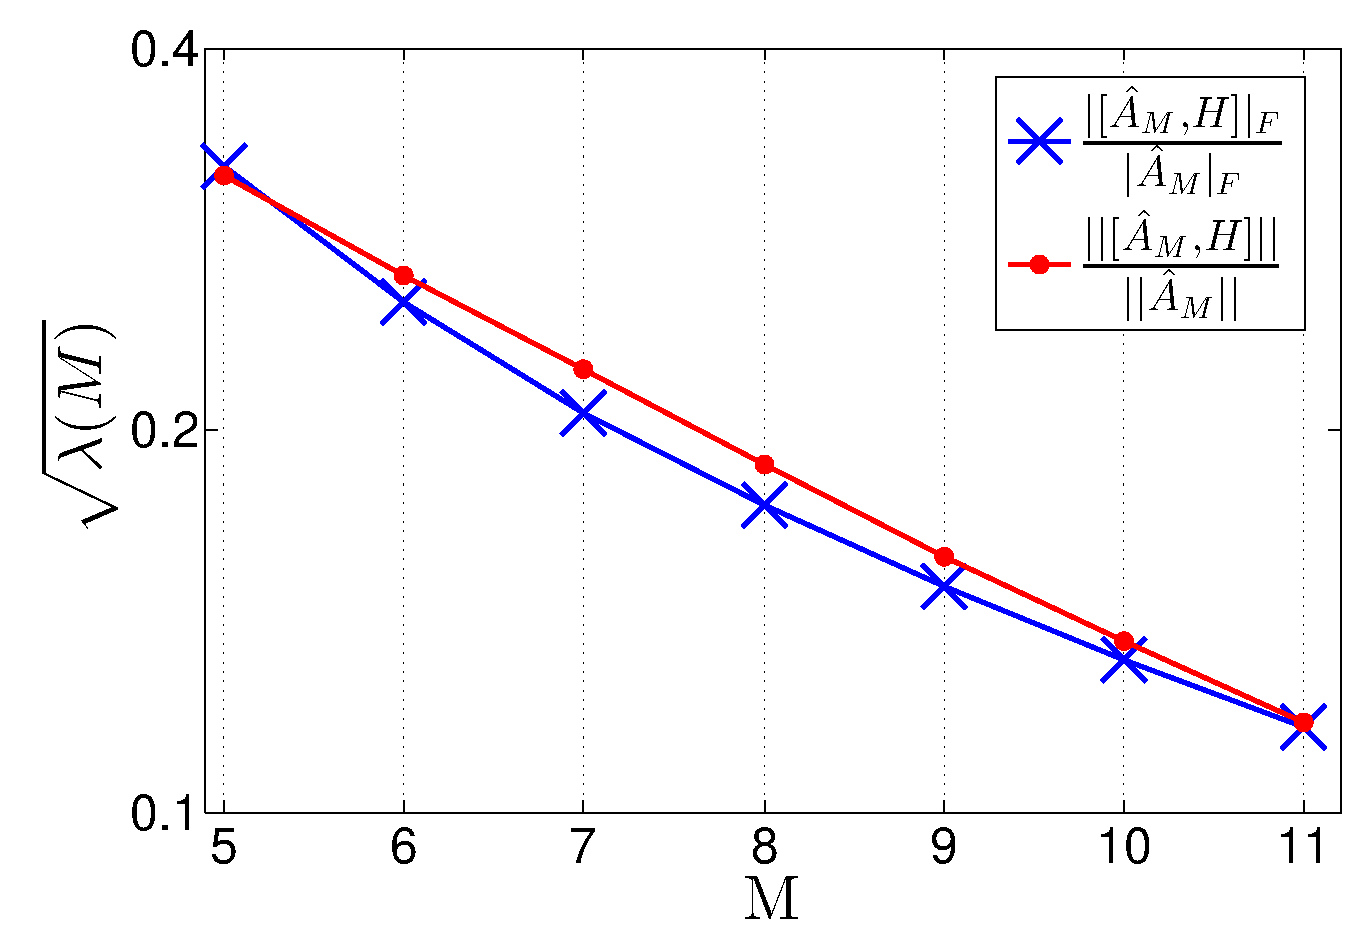
\includegraphics[width=1.0\linewidth]{infinite_ham_opnorm_modified.pdf}
\centering
\caption{(color online) Normalized magnitude of $[\hat{A}_M, H]$ measured by the Frobenius norm ($|\ldots|_F$) and the operator norm ($||\ldots||$)
in log-linear plot.
$\hat{A}_M$ is obtained by minimizing the Frobenius norm of the commutator with Hamiltonian as is in the main text.
Two norms give quantitatively similar values.
}
\label{fig:op_norm}
\end{figure}

For many purposes, the operator norm is mathematically more convenient
since we can directly interpret the relaxation of the operator in terms of Lieb-Robinson bounds \cite{Lieb:1972,Bravyi:2006}.
Optimizing the operator norm numerically is, however, very challenging. Therefore, we used the (square of) Frobenius norm in the main text.
Nevertheless, once we have an operator, it is easy to compute the operator norm of the commutator with Hamiltonian.
Figure \ref{fig:op_norm} plots the decay of the Frobenius norm and the operator norm of $[\hat{A}_M,H]$,
where $\hat{A}_M$ is obtained in the main text by minimizing the Frobenius norm.
It shows that the value of $\lambda$ measured by the operator norm is numerically similar to that of the Frobenius norm.
It appears that the operator norms computed for these operators exhibit exponential-like decrease with $M$ but
the range of $M$ is not enough to draw a conclusion.


\subsection{Results of another set of parameters}
\begin{figure}
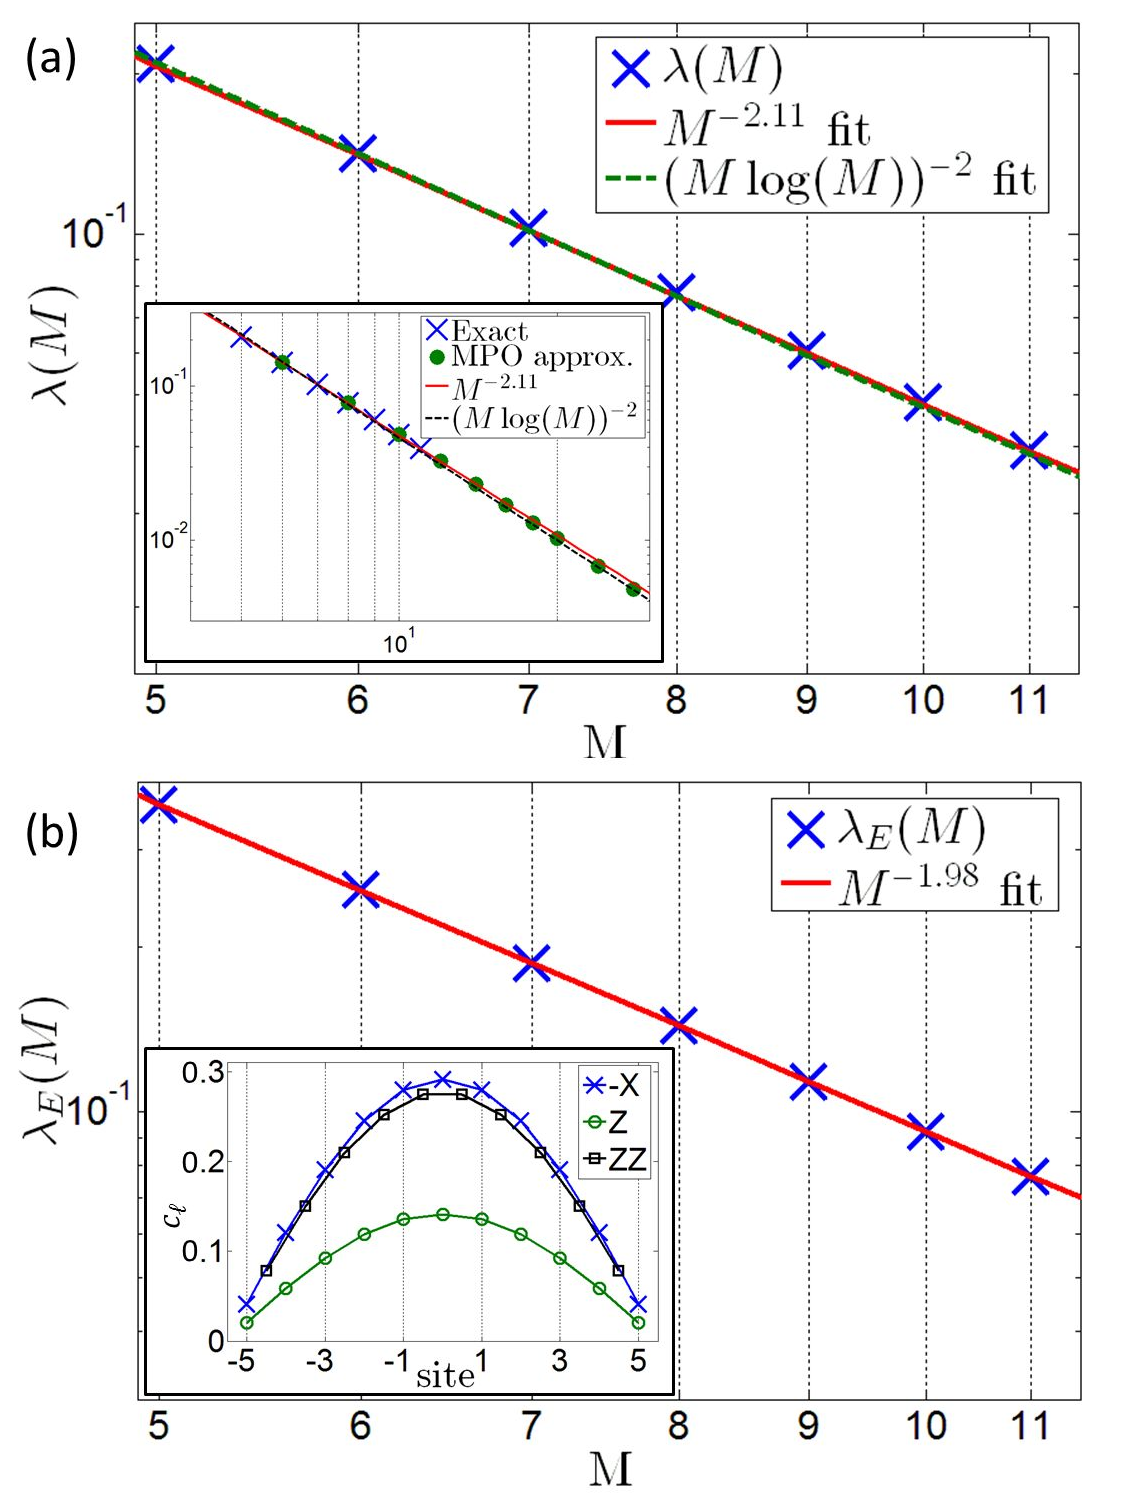
\includegraphics[width=1.0\linewidth]{fig_hamiltonian_modified_other.pdf}
\centering
\caption{(color online) (a) $\lambda(M)$ is the minimum value of the Frobenius norm of the commutator with Hamiltonian.
Here we choose the parameters to be $(g,h) = (-1.05, 0.5)$. $\lambda$ still decreases faster than $1/M^2$.
\addr{Inset: $\lambda(M)$ vs. $M$ using tensor network method (MPO approximation). The results are indistinguishable with available exact results.}
(b) $\lambda_E(M)$ is the same results when we restrict the search space within the terms in the Hamiltonian.
As expected, it has $M^{-2}$ scaling and the structure is cosine modulation (inset).}
\label{fig:hamiltonian_other}
\end{figure}
In this section, we show that the results in the main body do not depend on the parameter choice.
We choose another set of parameters $(g,h) = (-1.05, 0.5)$, which is the parameter choice of Ref.~\onlinecite{Banuls:2011}.

Figure \ref{fig:hamiltonian_other} (a) is the minimum value of Eq. \eqref{eq:minimize} with the other parameter choice.
We can see that it decays faster than $1/M^2$. As is the case of the parameter choice in the main body,
the data can be well-fitted by two methods; a power-law and a logarithmic correction to $1/M^2$.
Since the power-law exponent could depend on the parameter choice, we do not attempt to draw a strong conclusion from this data
except that $\lambda(M)$ decreases faster than $1/M^2$,
the scaling of the diffusive energy mode.

Figure \ref{fig:hamiltonian_other} (b) is the plot of the minimum value of Eq. \eqref{eq:minimize} when only terms in Hamiltonian are allowed
for two sets of parameters. Unlike the case where all operators are used,
the decay scaling remains the same as $1/M^2$ as expected from the hydrodynamics.
Therefore, we again explicitly demonstrate that the longest wavelength energy modulation is the slowest mode of a conserved quantity.


\subsection{Slow Operators for Arbitrary Quantum Circuits}

\begin{figure}
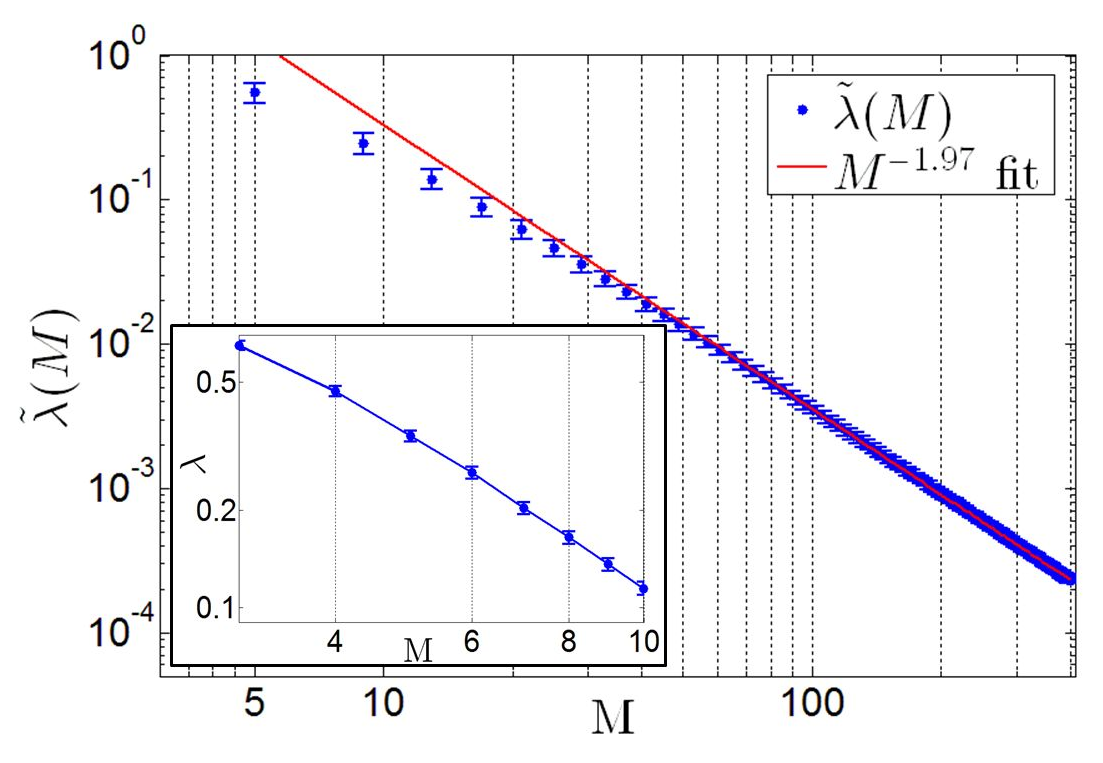
\includegraphics[width=1.0\linewidth]{fig_random_circuit.pdf}
\centering
\caption{ (color online)  $\tilde{\lambda}(M)$ for a random circuit model computed by matrix product method with the filtered of operators (Eq. \eqref{eq:filter}). $1/2\sigma^z$ is chosen for the single site Hermitian. We averaged 50 realizations of random circuits. Asymptotically, the data follows very closely $M^{-2}$.
Inset: $\lambda(M)$ is the result of exhaustive search without using the filtered form for the same model.
These values cannot be matched by the simple filtered operator we consider.}
\label{fig:random_circuit}
\end{figure}

\addr{ In the main body, we have shown that $\lambda(M)$ decreases as $M^{-2}$ for a Floquet system, where local conservation law is absent.}
To determine whether this phenomenon is more generally true, we also study a family of quantum circuits, each composed of two rounds, where in the first round, gates act on pairs of sites $...,(1,2),(3,4),...$ and on the second round gates act on pairs $...,(0,1),(2,3),(4,5),...$
We choose all gates in a given round to be the same, but choose them randomly.
The results are shown in Fig.~\ref{fig:random_circuit}.
We find again that even in this random case, slow operators are present.

We again apply the matrix product method to the same form of the operators, Eq. \eqref{eq:filter},
to study larger systems. Since our random circuit consists of two alternating non-commuting unitaries,
the support of $\tilde{A}_N$ is now $4N+1$ instead of $2N+1$.
In this random circuits, generally there is no single site Hermitian $\hat{O}$
that matches the exact calculation for a small system size, unlike in the Floquet operator we studied earlier.
Therefore, we just choose $\hat{O} = 1/2\sigma^z$ as a single site hermitian.
The weights $c_n$ again agree very well a cosine shape and $\lambda$ decays close to $1/M^2$.
This hints that $1/M^2$ would be a generic feature.


We now show that a slowly relaxing operator must always exist, on an interval of length $M$ with the relaxation rate going to zero as $M$ gets large.  Let $U$ be the unitary of the quantum circuit restricted to an interval of length slightly larger than $M$ (in this way, we can consider only finite dimensional spaces).

Let ${\cal E}(\hat{O})$ be a super-operator defined by ${\cal E}(\hat{O})=U\hat{O}U^\dagger$.  The space of operators can be regarded as a vector space, with inner product $(A,B)={\rm tr}(A^\dagger B)$, and with ${\cal E}(\hat{O})$ being a linear operator on this space.  The operator ${\cal E}$ is non-Hermitian but it is a normal operator, since its Hermitian conjugate is equal to ${\cal E}^\dagger(\hat{O})=U^\dagger \hat{O} U$ and ${\cal E}({\cal E}^\dagger(\hat{O}))={\cal E}^\dagger({\cal E}(\hat{O}))=\hat{O}$ and so $[{\cal E},{\cal E}^\dagger]=0$.
Let ${\cal E}_h=\frac{1}{2}({\cal E}+{\cal E}^\dagger)$ and ${\cal E}_a=\frac{1}{2i}({\cal E}-{\cal E}^\dagger)$.

We begin by constructing an operator $\hat{O}$ supported on an interval of length $M$ such that ${\cal E}_h(\hat{O})= x \hat{O}+\hat{\epsilon}$ for some $x$ and for $\hat{\epsilon}={\cal O}(1/M)$.  Let $A$ be any traceless operator supported on a single site in the center of the interval.  We consider the Krylov space generated by the vectors $A, {\cal E}_h(A), {\cal E}_h^2(A),...$.  Let $K$ be the number of vectors we take; $K$ will be proportional to $M$ and will be chosen such that all these operators are supported on the interval of length $M$.
Since ${\cal E}_h$ is Hermitian, using the Lanczos procedure we can write it as a tridiagonal matrix $T$ in this Krylov space.   We claim that that there exists a vector $v$ supported on the first $K-1$ vectors $w_1,...,w_{K-1}$ such that $|Tv-xv|^2/|v|^2\leq {\cal O}(1/K^2)$.  To verify this claim, let $\psi$ be any eigenvector of $T$ with at least half its weight on the first $K/2$ vectors with $\psi=\sum_k a_k v_k$; let $x$ be the corresponding eigenvalue; let $v=\sum_k a_k (1-k/K) v_k$.
The basis in which the matrix is tridiagonal has basis vectors $w_1,w_2,...$, with $w_k$ being in the span of the first $k$ vectors $A, {\cal E}_h(A),...$
Hence, the vector $v$ gives us the desired operator $\hat{O}$.

Now consider the operators
\be
\hat{O}_{\pm}=(\sqrt{1-x^2} \pm {\cal E}_a) \hat{O},
\ee
with $\hat{O}$ normalized such that $||\hat{O}||=1$.
Note that ${\cal E}(\hat{O}_{\pm})={\cal E}_h(\hat{O}_{\pm})+i {\cal E}_a(\hat{O}_{\pm})=x\hat{O}_{\pm}+i(\sqrt{1-x^2}{\cal E}_a \pm {\cal E}_a^2) \hat{O} + {\cal O}(1/M)$.  Using
the fact that ${\cal E}_h^2+{\cal E}_a^2$ is equal to the identity super-operator, $(\sqrt{1-x^2}{\cal E}_a \pm {\cal E}_a^2) \hat{O}=\sqrt{1-x^2}{\cal E}_a \pm (1-x^2) ) \hat{O} +{\cal O}(1/M)=\pm\sqrt{1-x^2}\hat{O}_{\pm}+{\cal O}(1/M)$.
Hence,
\be
{\cal E}(\hat{O}_{\pm})=z \hat{O}_{\pm}+{\cal O}(1/M)
\ee
with
\be
z=x\pm i \sqrt{1-x^2},
\ee
so that $|z|=1$.
At least one of the two operators $\hat{O}_{\pm}$ must have non-negligible norm.  Let $X$ be the corresponding operator, normalized to have norm $1$.  Hence, we have constructed an operator $X$ supported on the interval of length $M$ such that ${\cal E}(X)=z X + {\cal O}(1/M)$.

This already implies that there is some operator $X$ which is slowly relaxing but perhaps oscillating; i.e., since $X$ is an approximate eigenoperator of ${\cal E}$, if $z=1$ then $X$ changes slowly over time, while if $z \neq 1$, then the expectation value of $X$ oscillates.

In fact, we can always construct an operator $Y$ which is an approximate eigenoperator of ${\cal E}$.  Here is one way.  Consider many disjoint intervals of length $M$.  Let $X_1,X_2,...$ be the operators on these intervals with eigenvalues $z_1,z_2,...$  Choose some subset $S$ of these intervals such that the product of the $z_i$ on that subset is close to $1$: $\prod_{i \in S} z_i \approx 1$.  Then, let $Y=\prod_{i \in S} X_i$.  This requires some analytic estimates to determine the support of $Y$ required: since $Y$ is a product of many operators, the error (in that each $X_i$ is only an approximate eigenoperator) may add, so the support of $Y$ may scale as a fairly large polynomial in the error.  We leave this estimate for later.

\subsection{$1/M^2$ scaling of filtered operators}
We show $1/M^2$ scaling of filtered operators of the form Eq. \eqref{eq:filter} if $\mathrm{tr}(\hat{O}U^n \hat{O}U^{-n}) = 0$ for all $n\neq 0$,
where $\hat{O}$ is a traceless Hermitian acting on a single site.
First, observe that
\begin{align}
& \frac{\mathrm{tr}([\tilde{A}_N,U][\tilde{A}_N,U])}{\mathrm{tr}(\tilde{A}_N\tilde{A}_N^\dag)} \nonumber\\
&=2 - \bigg(\sum_{n,m = -N}^{N}c_n c_m \mathrm{tr}(U^{n-m-1}\hat{O}U^{-n+m+1}\hat{O} \nonumber\\
&\quad\quad\quad\quad\quad + U^{n-m+1}\hat{O}U^{-n+m-1}\hat{O})\bigg)/\mathrm{tr}(\tilde{A}_N\tilde{A}_N^\dag) ~.
\end{align}
Therefore, if $\mathrm{tr}(\hat{O}U^n \hat{O}U^{-n}) = \delta_{n,0}\mathrm{tr}(\hat{O}\hat{O}^\dag)$,
the above expression simplifies to
\begin{align}
\frac{\mathrm{tr}([\tilde{A}_N,U][\tilde{A}_N,U])}{\mathrm{tr}(\tilde{A}_N\tilde{A}_N^\dag)}=2\left(1 - \frac{\sum_{n=-N}^{N-1}c_n c_{n+1}}{\sum_{n=-N}^N c_n^2}\right) ~.
\end{align}
This is a trivial quadratic optimization problem and the solution is $c_n = \cos(n\pi/(2N+2))$.
Therefore, the minimum value $\tilde{\lambda}$ for sufficiently large $N$ is
\begin{align}
\tilde{\lambda} &= \mathrm{min}\left[\frac{\mathrm{tr}([\tilde{A}_N,U][\tilde{A}_N,U])}{\mathrm{tr}(\tilde{A}_N\tilde{A}_N^\dag)} \right] \nonumber\\
&= 2 - 2\cos\left(\frac{\pi}{2N+2}\right) \simeq \frac{\pi^2}{4(N+1)^2} \sim \frac{1}{M^2} ~,
\end{align}
where we used the fact that the support $M = 4N +1 $.


Ref. ~\onlinecite{Kim_ETH} has shown that the $U_F$ (Eq. \eqref{eq:floquet_op}) thermalizes a local operator at infinite temperature,
and thus $\mathrm{tr}(\hat{O}U^n\hat{O}U^{-n}) = 0$ for a sufficiently large $n$.
For the Floquet system, therefore, the above condition is approximately satisfied for a large enough $N$.
Figure \ref{fig:floquet} shows that for $N$ = 60 and 100, the form is very close to the cosine
and the scaling for large $M = 2N +1$ closely follows $M^{-2}$ scaling.
For a general random circuit, Figure \ref{fig:random_circuit} again shows $M^{-2}$ scaling. The structure of $\{c_n\}$
is found to follow cosine modulation similar to the Floquet case (not shown).

One example of quantum circuits that satisfies the condition that $\mathrm{tr}(\hat{O}U^{n} \hat{O}U^{-n}) = 0$ for all $n\neq0$
is the swap operator $U_{sw}$.
\begin{align}
U_{sw} = \prod_n V_{2n,2n+1} \prod_m V_{2m-1,2m} ~,
\end{align}
where $V_{x,y}$ swaps the spins ${\bf S}_x$ and ${\bf S}_y$; $V_{x,y}|{\bf S}_x,{\bf S}_y\rangle = |{\bf S}_y, {\bf S}_x\rangle$.
Then, for an $\hat{O}$ acting on site 0, $U_{sw}$ moves $\hat{O}$ to the site $-2n$ and $U_{sw}^{-n}$ moves $\hat{O}$ to the site $2n$
and thus the condition is satisfied.
In this case, we can write every step analytically and prove $1/M^2$ scaling and the cosine modulation.
In a generic quantum circuit, however, these features are seen only for sufficiently large $M$.
Furthermore, in a translation invariant system, $U_{sw}$ has an exact local conservation law.
For instance, any translation invariant single site operator commutes with $U_{sw}$ and thus conserved.

In the main text, we connected $\lambda(M)$ to the thermalization time scale by $1/\tau \sim \sqrt{\lambda(M)}$ (Eq. \eqref{eq:floquet_timescale}).
At first glance, $1/\tau \sim \sqrt{\lambda(M)} \sim 1/M$ may seem trivial for an operator of support $M$ by Lieb-Robinson bound type argument,
but an important point here is that we computed the relaxation of an operator by the Frobenius norm,
not the operator norm by which the Lieb-Robinson bound has been computed \cite{Lieb:1972}.

\end{document}
